\documentclass[12pt]{beamer}
% \usepackage[top=1in, left=1in, right=1in, bottom=1in]{geometry}
\usepackage{graphicx}
\usepackage{tikz}
\usetikzlibrary{graphs, shapes, arrows}
\usepackage[sorting=none]{biblatex}
\addbibresource{sample.bib}

\usecolortheme{beaver}
\definecolor{xred}{HTML}{a30000}
\definecolor{myblue}{HTML}{00a1e5}
\setbeamercolor{titlelike}{parent=structure,fg=white,bg=xred}
\setbeamercolor{frametitle}{fg=white,bg=xred}
\setbeamercolor{section in toc}{fg=xred}
\setbeamerfont{frametitle}{size=\linespread{0.7}\selectfont}
\setbeamertemplate{frametitle}[default][center]
\setbeamertemplate{navigation symbols}{}

% \setbeamertemplate{sections/subsections in toc}[sections numbered]
\setbeamertemplate{section in toc}{\hspace*{1em}\inserttocsection}
\setbeamertemplate{subsection in toc}{\hspace*{2em}\inserttocsubsection}
\setbeamertemplate{itemize item}{\color{black}$\blacktriangleright$}

% FOOTER CHANGE
\makeatother
\setbeamertemplate{footline}
{
	\leavevmode%
	\hbox{%
		
		\begin{beamercolorbox}[wd=0.9\paperwidth,ht=2.25ex,dp=1ex,left]{date in head/foot}%
			\hspace{1em}
			% \insertframetitle{}
			\insertsectionhead{}
		\end{beamercolorbox}%
		
		\begin{beamercolorbox}[wd=0.1\paperwidth,ht=2.25ex,dp=1ex,right]{title in head/foot}%
			\usebeamerfont{title in head/foot} 
			\insertframenumber{} / \inserttotalframenumber{}
			\hspace{1em}
		\end{beamercolorbox}
	}%
	\vskip0pt%
}% 
\makeatletter

% meta-data
\title{Graph Coloring}
\subtitle{Exact and Approximate Algorithms}
\author{1705039 , 1705044 \\ \textit{\vspace*{-2cm}Group-7}}
\date[]{}

%FIXING TITLEPAGE
% \title{Class on LaTeX: Beamer}

% \subtitle{An Introduction}

% \author[M. Nahar]{Mahjabin Nahar}
% %\author{A.~B \and X.~Y}

% \institute[CSE, BUET]
% {
%   Department of Computer Science and Engineering\\
%   Bangladesh University of Engineering and Technology
% }

% \date{\today}

% \logo{\includegraphics[height=1cm]{overleaf.png}}

% PLACING ToC AT THE BEGINNING OF EACH SECTION
\AtBeginSection[]
{{
		\setbeamercolor{background canvas}{bg=gray!10}
		\setbeamertemplate{footline}{} 
		\begin{frame}
			\frametitle{}
			\centering
			\Large
			\tableofcontents[currentsection]
		\end{frame}
}}


\tikzset{
	every node/.style={line width=1.2pt,fill=white,shape=circle,draw=black},
	every edge/.style={line width=1.2pt,draw=black},
	box/.style={shape=rectangle,line width=1pt},
	red-node/.style={fill=red!70},
	blue-node/.style={fill=blue!50},
	green-node/.style={fill=green!70},
	yellow-node/.style={fill=yellow!70},
	cyan-node/.style={fill=cyan!70},
	invisible/.style={draw=none,fill=none,opacity=0},
	highlight/.style={font=\bfseries, inner sep = 3.65pt, line width=1.5pt, fill=gray!20},
	red-on/.style={alt={#1{red-node}{}}},
	blue-on/.style={alt={#1{blue-node}{}}},
	green-on/.style={alt={#1{green-node}{}}},
	yellow-on/.style={alt={#1{yellow-node}{}}},
	cyan-on/.style={alt={#1{cyan-node}{}}},
	invisible-on/.style={alt={#1{invisible}{}}},
	highlight-on/.style={alt={#1{highlight}{}}},
	alt/.code args={<#1>#2#3}{
		\alt<#1>{\pgfkeysalso{#2}}{\pgfkeysalso{#3}}
	}
}

\tikzstyle{startstop} = [ellipse,  minimum width=1cm, minimum height=1cm,text centered, draw=black]
\tikzstyle{io} = [trapezium, trapezium left angle=70, trapezium right angle=110, minimum width=3cm, minimum height=1cm, text centered, draw=black]
\tikzstyle{process} = [rectangle, minimum width=3cm, minimum height=1cm, text centered, draw=black]
\tikzstyle{decision} = [diamond, aspect=3, minimum width=1cm, minimum height=1.5cm,text centered,draw=black]
\tikzstyle{label} = [draw=none,fill=none]
\tikzstyle{arrow} = [thick,->,>=stealth]
\tikzstyle{flow-highlight} = [fill=blue!30,text=black]
\tikzstyle{flow-highlight-on} = [alt={#1{flow-highlight}{}}]

% \defbeamertemplate*{title page}{customized}[1][]
% {
%     \centering 
%     \usebeamerfont{title}\inserttitle\par
%     \usebeamerfont{subtitle}\insertsubtitle\par

%     \bigskip
%     \bigskip
%     \usebeamerfont{author}\insertauthor\par
%     \usebeamerfont{author}{(Group 7)}\par
% }

% ============================= DOCUMENT ================================

\begin{document}
	
	{
		\setbeamercolor{background canvas}{bg=gray!10}
		\setbeamertemplate{navigation symbols}{}
		\setbeamertemplate{footline}{} 
		\begin{frame}
			\titlepage
		\end{frame}
	}
	
	%FRAME AND FIGURE
	%\begin{frame}{Frame 1}
	%This is some text in the first frame. 
	%\end{frame}
	%
	%\begin{frame}{Frame 2}
	%\begin{figure}[h]
	%	\centering
	%	\includegraphics[scale=0.4]{graph.png}
	%	\caption{This caption is at the bottom}
	%	\label{fig:1}
	%	%\caption{This is figure 1.}
	%\end{figure}
	%\end{frame}
	
	%TABLE OF CONTENTS
	
	
	\section{Problem Statement}
	\begin{frame}{Basic Definitions}
		Assign colors to \emph{certain elements} of a graph subject to \emph{certain constraints} \vspace{20pt}\pause
		
		\textbf{Vertex coloring} is the most common graph coloring problem. \vspace{20pt}\pause
		
		\centering
		\emph{"A way of coloring the vertices of a graph such that no two adjacent vertices are of the same color."} 
	\end{frame}
	
	\begin{frame}{Trivial Solution}
		\begin{columns}
			\column{0.5\textwidth}
			\centering
			Assign new colors \\ 
			for every vertex
			
			\column{0.5\textwidth}
			\begin{figure}[h]
				\centering
				
				\resizebox{0.7\linewidth}{!}{
					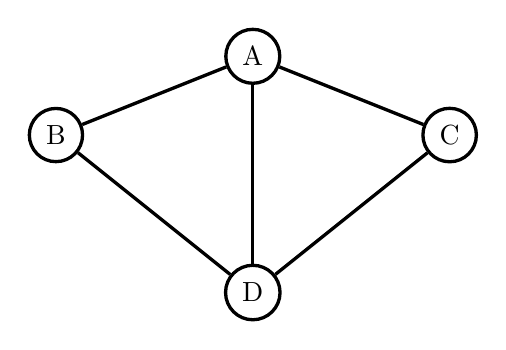
\begin{tikzpicture}
					\node[red-on=<1->] (A) at (2.5,5) {A};
					\node[blue-on=<1->] (B) at (0,4) {B};
					\node[yellow-on=<1->] (C) at (5,4) {C};
					\node[green-on=<1->] (D) at (2.5,2) {D};
					
					\path [-] (A) edge (B);
					\path [-] (A) edge (C);
					\path [-] (A) edge (D);
					\path [-] (B) edge (D);
					\path [-] (D) edge (C);
					
					\end{tikzpicture}}
				
				\label{fig:1}
				\caption{4 colors}
			\end{figure}
			
		\end{columns}
	\end{frame}
	
	\begin{frame}{Chromatic Number}
		\begin{columns}
			\column{0.5\textwidth}
			\centering
			Find the minimum colors \\
			(\textit{chromatic number}) \\ 
			
			\column{0.5\textwidth}
			\begin{figure}[h]
				\centering
				
				\resizebox{0.7\linewidth}{!}{
					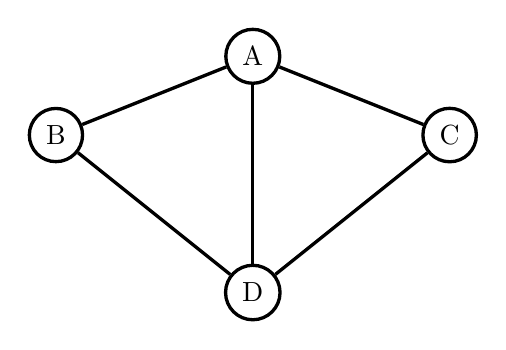
\begin{tikzpicture}
					\node[red-on=<1->] (A) at (2.5,5) {A};
					\node[blue-on=<1->] (B) at (0,4) {B};
					\node[blue-on=<1->] (C) at (5,4) {C};
					\node[green-on=<1->] (D) at (2.5,2) {D};
					
					\path [-] (A) edge (B);
					\path [-] (A) edge (C);
					\path [-] (A) edge (D);
					\path [-] (B) edge (D);
					\path [-] (D) edge (C);
					
					\end{tikzpicture}}
				
				\label{fig:2}
				\caption{3 colors}
			\end{figure}
			
		\end{columns}
	\end{frame}
	
	\section{Solution Overview}
	\begin{frame}{Computational Complexity}
		\begin{columns}
			\column{0.5\textwidth}
			\begin{figure}[h]
				\centering
				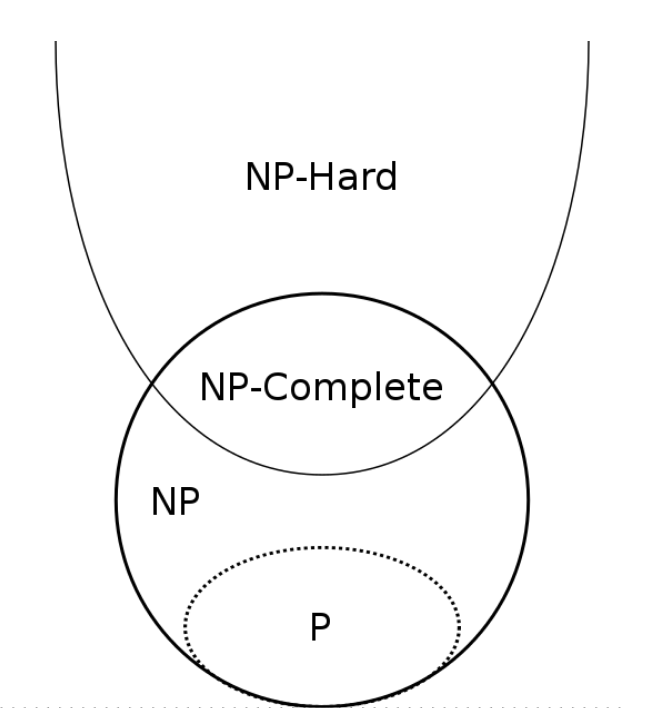
\includegraphics[scale=0.5,width=0.8\linewidth]{diagrams/diagram-3.png}
				\label{fig:3}
			\end{figure}
			
			
			\column{0.5\textwidth}
			\centering	
			
			Decision problem \\ 
			\textit{(is the graph k-colorable?)} \\
			is \textbf{NP-Complete}. \\ \vspace{30pt} \pause
			
			Optimization problem \\ 
			\textit{(find minimum colors k)} \\
			is \textbf{NP-Hard}.
		\end{columns}
	\end{frame}
	
	\begin{frame}{Algorithms}
		\begin{columns}
			\column{0.55\textwidth}
			\centering
			\large
			\textbf{Approximate algorithm}
			\normalsize \vspace{10pt}
			\begin{itemize}
				\item Greedy method
				\item Solvable in limited time
				\item May not yield minimum
			\end{itemize}
			
			\pause
			
			\column{0.45\textwidth}
			\centering
			\large
			\textbf{Exact algorithm}
			\normalsize \vspace{10pt}
			\begin{itemize}
				\item Dynamic Programming
				\item Minimum guaranteed
				\item Under constraints
			\end{itemize}
		\end{columns}
	\end{frame}
	
	\section{Greedy Algorithm}
	
	\begin{frame}{Basic Idea}	
		Make \emph{locally optimal choice} at each step \vspace{20pt}
		
		\textbf{Greedy choice:} \textit{Using existing colors} \vspace{20pt}\pause
		
		\begin{itemize}
			\item Reuse a color $k$
			\begin{equation}
			\label{eqn:1}
			V_i.color = k : (k \in C) \hspace{5pt} \& \hspace{5pt} (k \not\in \varepsilon)
			\end{equation}
			\pause
			
			\item If colors are exhausted
			\begin{equation}
			\begin{aligned}
			\label{eqn:2}
			V_i.co&lor = k : (k \not\in C) \\
			C & = C \cup \{k\}
			\end{aligned}
			\end{equation}
		\end{itemize}
	\end{frame}
	
	\begin{frame}{Simulation}
		\begin{columns}
			
			\begin{column}{0.5\textwidth}
				\begin{figure}
					% \centering
					\resizebox{0.7\linewidth}{!}{
						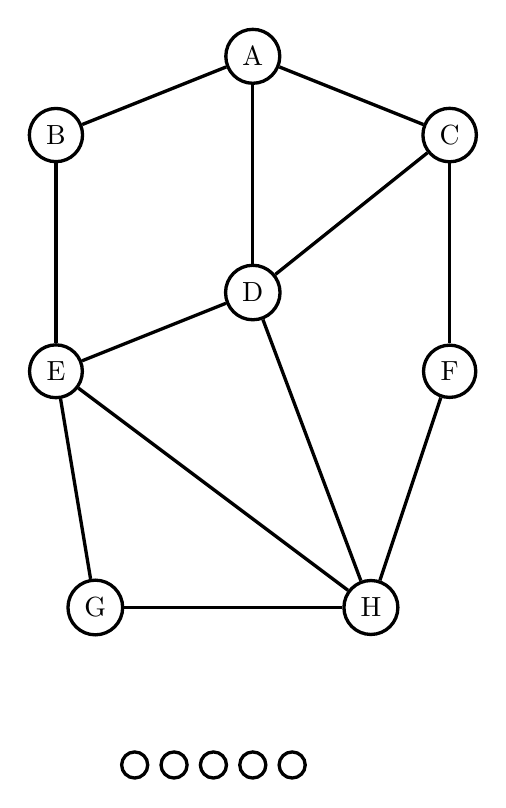
\begin{tikzpicture}
						\node[highlight-on=<2-3>,red-on=<3->] (A) at (2.5,5) {A};
						\node[highlight-on=<2-3>, highlight-on=<8-9>, blue-on=<5->] (B) at (0,4) {B};
						\node[highlight-on=<2-3>, blue-on=<6->] (C) at (5,4) {C};
						\node[highlight-on=<2-3>, highlight-on=<8-9>, green-on=<7->] (D) at (2.5,2) {D};
						\node[highlight-on=<8-9>, red-on=<9->] (E) at (0,1) {E};
						\node[red-on=<12->] (F) at (5,1) {F};
						\node[highlight-on=<8-9>, green-on=<11->] (G) at (0.5,-2) {G};
						\node[highlight-on=<8-9>, blue-on=<10->] (H) at (4, -2) {H} ;
						
						% color array
						\node[red-on=<3->] () at (1,-4) {};
						\node[blue-on=<5->] () at (1.5,-4) {};
						\node[green-on=<7->] () at (2,-4) {};
						\node[] () at (2.5,-4) {};
						\node[] () at (3,-4) {};
						
						\path [-] (E) edge (B);
						\path [-] (B) edge (A);
						\path [-] (E) edge (D);
						\path [-] (D) edge (A);
						\path [-] (E) edge (G);
						\path [-] (D) edge (C);
						\path [-] (A) edge (C);
						\path [-] (H) edge (G);
						\path [-] (H) edge (E);
						\path [-] (H) edge (D);
						\path [-] (F) edge (C);
						\path [-] (F) edge (H);
						
						
						\end{tikzpicture}
					}
				\end{figure}
			\end{column}
			% \hspace{-50pt}
			{\color{gray!20!white}\vrule{}}
			
			\begin{column}{0.5\textwidth}
				\resizebox{0.9\linewidth}{!}{
					\centering
					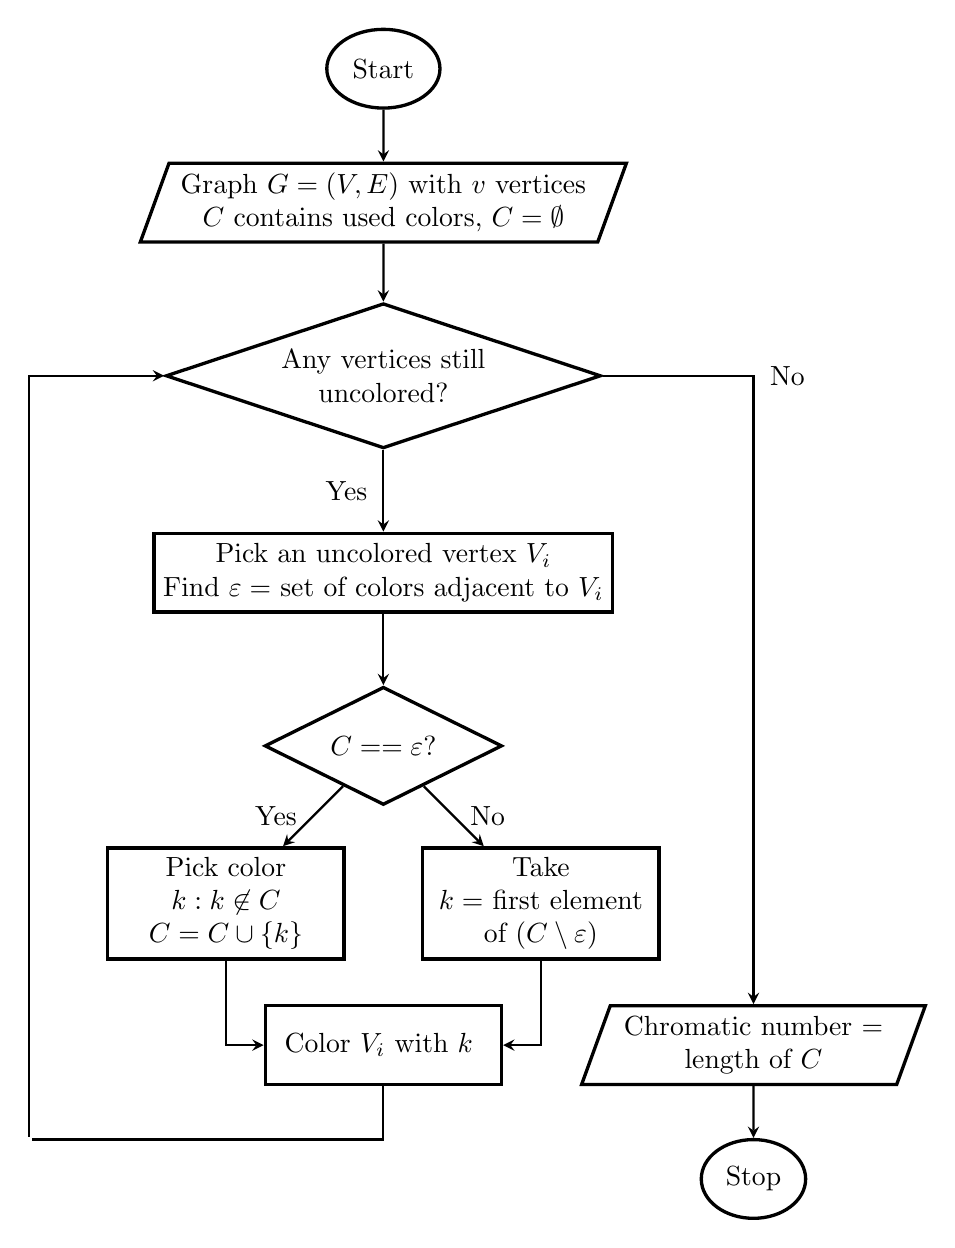
\begin{tikzpicture}
					
					\node[startstop, flow-highlight-on=<1>, %flow-highlight-on=<5-7>, flow-highlight-on=<10->
					] (start) {Start};
					
					\node[io, flow-highlight-on=<1>, %flow-highlight-on=<5-7>,flow-highlight-on=<10->, 
					below of = start, align=center, yshift=-0.7cm] (in) {
						Graph $G = (V,E)$ with $v$ vertices \\
						$C$ contains used colors, $C = \emptyset$
					};
					
					\node[decision, flow-highlight-on=<2>, flow-highlight-on=<4-8>, flow-highlight-on=<10->, below of = in, yshift=-1.2cm, align=center] (exit_con) {Any vertices still\\ uncolored?};
					
					\node[process, flow-highlight-on=<2>, flow-highlight-on=<5-8>, flow-highlight-on=<10-11>, below of = exit_con, yshift = -1.5cm, align=center] (pick_v) {
						Pick an uncolored vertex $V_i$ \\ 
						Find $\varepsilon = $ set of colors adjacent to $V_i$
					};
					
					\node[decision, flow-highlight-on=<3>, flow-highlight-on=<5-7>, flow-highlight-on=<9-11>, below of = pick_v, yshift = -1.2cm] (color_check) {$C==\varepsilon?$};
					
					\node[process, flow-highlight-on=<3>, flow-highlight-on=<5>, flow-highlight-on=<7>, below of = color_check, yshift = -1.0cm, xshift = -2cm, align=center] (new_color) {
						Pick color \\
						$k : k \not\in C$ \\
						$C=C \cup \{k\} $
					};
					
					\node[process, flow-highlight-on=<6>, flow-highlight-on=<9-11>, below of = color_check, yshift = -1.0cm, xshift = 2cm, align=center] (old_color) {
						Take \\
						$k = $ first element \\
						of $\left(C \setminus \varepsilon \right)$
					};
					
					\node[process, flow-highlight-on=<3>, flow-highlight-on=<5-7>, flow-highlight-on=<9-11>, below of = color_check, yshift = -2.8cm, align=center] (color) {
						Color $V_i$ with $k$
					};
					
					\node[label, left of = color, xshift = -3.5cm, yshift=-1.2cm, inner sep=0] (left) {
					};
					
					\node[io, flow-highlight-on=<12>, right of = color, xshift = 3.7cm,, align=center] (out) {
						Chromatic number = \\
						length of $C$
					};
					
					\node[startstop, flow-highlight-on=<12>, below of = out, yshift=-0.7cm] (exit) {Stop};
					
					\draw[arrow] (start) -- (in);
					\draw[arrow] (in) -- (exit_con);
					\draw[arrow] (exit_con) -| node[label,right] {No} (out);
					\draw[arrow] (exit_con) -- node[label, left] {Yes} (pick_v);
					\draw[arrow] (pick_v) -- (color_check);
					\draw[arrow] (color_check) -- node[label,left] {Yes} (new_color);
					\draw[arrow] (color_check) -- node[label, right] {No} (old_color);
					\draw[arrow] (new_color) |- (color);
					\draw[arrow] (old_color) |- (color);
					\draw[arrow, -] (color) |- (left);
					\draw[arrow] (left) |- (exit_con);
					\draw[arrow] (out) -- (exit);
					\end{tikzpicture}
				}
			\end{column}
		\end{columns}
		
	\end{frame}
	
	\begin{frame}{Complexity \& Limitations}
		\begin{itemize}
			\item Time Complexity : $O(V^2 + E)$\pause \vspace{10pt}
			\item Doesn't guarantee minimum number of colors\pause \vspace{10pt}
			\item Upper bound of $d+1$ where $d$ is maximum degree
		\end{itemize}
	\end{frame}
	
	\section{Dynamic Programming}
	
	\begin{frame}{Basic Idea}	
		Combine \textit{solutions of sub-problems} \vspace{20pt} \pause
		
		\textbf{Apply:} Chromatic number of a graph is derived from its sub-graphs \vspace{20pt}
		
		\begin{figure}[h]
			\centering
			
			\resizebox{0.4\linewidth}{!}{
				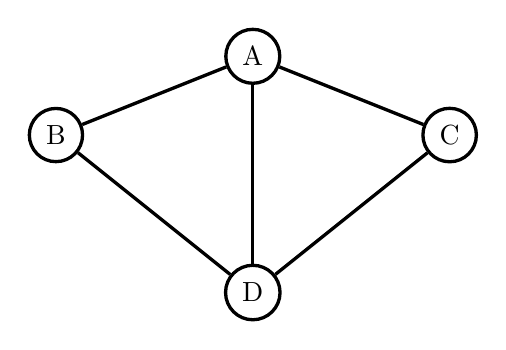
\begin{tikzpicture}
				\node[red-on=<3>, red-on=<7>] (A) at (2.5,5) {A};
				\node[blue-on=<4>, blue-on=<6-7>] (B) at (0,4) {B};
				\node[blue-on=<5-7>] (C) at (5,4) {C};
				\node[green-on=<5>, green-on=<7>] (D) at (2.5,2) {D};
				
				\path [-] (A) edge (B);
				\path [-] (A) edge (C);
				\path [-] (A) edge (D);
				\path [-] (B) edge (D);
				\path [-] (D) edge (C);
				
				\end{tikzpicture}}
			
			\label{fig:dp_sub}
		\end{figure}
		
	\end{frame}
	\begin{frame}{Basic Idea}
		\textbf{Idea:} A \textit{maximal independent set} is 1-colorable \vspace{20pt} \pause
		
		\textbf{Solution:} \\ 
		\hspace{80pt}
		$\chi (G[S]) = 1 + \chi (G[S \setminus I]) $
		\vspace{20pt}
		% 		\vspace{20pt}
		%		\chi (G[S]) = 1 + min \{ \chi (G[S \setminus I]): i \in I(G[S]) \}
		
		\begin{figure}[h]
			\centering
			
			\resizebox{0.4\linewidth}{!}{
				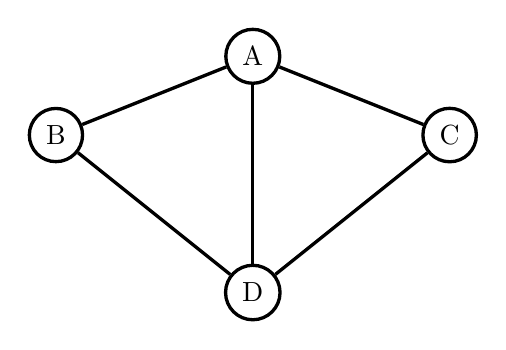
\begin{tikzpicture}
				\node[red-on=<4->] (A) at (2.5,5) {A};
				\node[highlight-on=<3>, blue-on=<5->] (B) at (0,4) {B};
				\node[highlight-on=<3>, blue-on=<5->] (C) at (5,4) {C};
				\node[green-on=<4->] (D) at (2.5,2) {D};
				
				\path [-] (A) edge (B);
				\path [-] (A) edge (C);
				\path [-] (A) edge (D);
				\path [-] (B) edge (D);
				\path [-] (D) edge (C);
				
				\end{tikzpicture}}
			
			\label{fig:dp_SI}
		\end{figure}
		
		\onslide<6->{
			\textit{But there is a catch!}
		}
	\end{frame}
	
	\begin{frame}{Simulation}
		\begin{columns}
			
			\begin{column}{0.5\textwidth}
				\begin{figure}
					% \centering
					\resizebox{0.7\linewidth}{!}{
						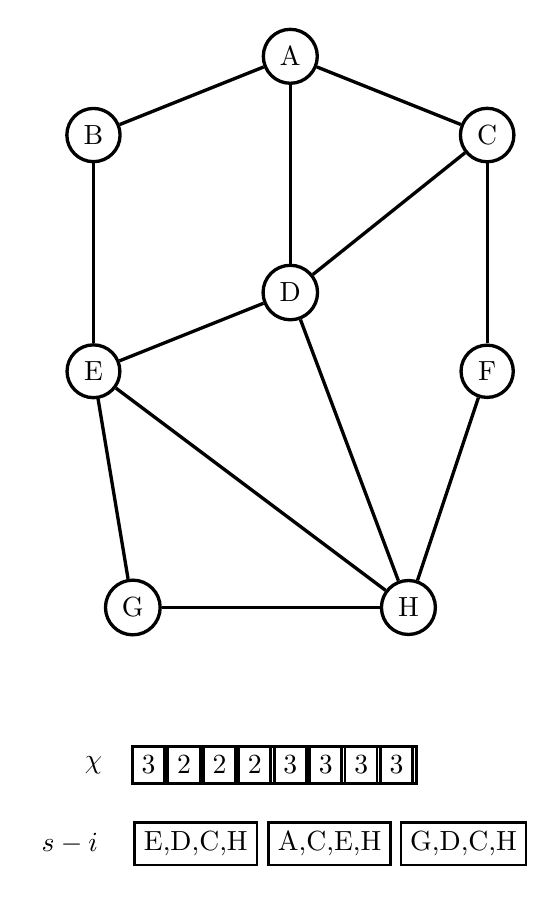
\begin{tikzpicture}
						\node[highlight-on=<2-8>,blue-on=<3-4>, green-on=<6>,
						blue-on=<7-8>, green-on=<9>] (A) at (2.5,5) {A};
						\node[blue-on=<9>] (B) at (0,4) {B};
						\node[highlight-on=<2-8>, red-on=<4>, red-on=<6>, red-on=<8-9>] (C) at (5,4) {C};
						\node[highlight-on=<2-8>, green-on=<4>, blue-on=<5-6>, green-on=<8>, blue-on=<9>] (D) at (2.5,2) {D};
						\node[highlight-on=<2-8>, red-on=<4>, red-on=<6>, blue-on=<7-8>, red-on=<9>] (E) at (0,1) {E};
						\node[highlight-on=<2-8>,blue-on=<3-9>] (F) at (5,1) {F};
						\node[highlight-on=<2-8>, blue-on=<3-6>, green-on=<8>, blue-on=<9>] (G) at (0.5,-2) {G};
						\node[highlight-on=<2-8>, cyan-on=<4>, green-on=<6>, red-on=<8>, green-on=<9>] (H) at (4, -2) {H} ;
						
						% X array
						\node[label] () at (0,-4) {$\chi$};
						\node[box,blue-on=<3-4>] () at (0.7,-4) {3};
						\node[box,blue-on=<5-6>] () at (1.15,-4) {2};
						\node[box,blue-on=<7-8>] () at (1.60,-4) {2};
						\node[box] () at (2.05,-4) {2};
						\node[box,invisible-on=<4->] () at (2.50,-4) {X};
						\node[box,red-on=<4->,invisible-on=<1-3>,invisible-on=<6->] () at (2.50,-4) {4};
						\node[box,red-on=<4-8>,invisible-on=<-5>] () at (2.50,-4) {3};
						\node[box,invisible-on=<9>] () at (2.95,-4) {X};
						\node[box,invisible-on=<-8>] () at (2.95,-4) {3};
						\node[box,invisible-on=<9>] () at (3.40,-4) {X};
						\node[box,invisible-on=<-8>] () at (3.40,-4) {3};
						\node[box,invisible-on=<9>] () at (3.85,-4) {X};
						\node[box,red-on=<9>,invisible-on=<-8>] () at (3.85,-4) {3};
						
						% S - I array
						\node[label] () at (-0.3,-5) {$s-i$};
						\node[box,blue-on=<3-4>] () at (1.3,-5) {E,D,C,H};
						\node[box,blue-on=<5-6>] () at (3.0,-5) {A,C,E,H};
						\node[box,blue-on=<7-8>] () at (4.7,-5) {G,D,C,H};
						
						\path [-] (E) edge (B);
						\path [-] (B) edge (A);
						\path [-] (E) edge (D);
						\path [-] (D) edge (A);
						\path [-] (E) edge (G);
						\path [-] (D) edge (C);
						\path [-] (A) edge (C);
						\path [-] (H) edge (G);
						\path [-] (H) edge (E);
						\path [-] (H) edge (D);
						\path [-] (F) edge (C);
						\path [-] (F) edge (H);
						
						
						\end{tikzpicture}
					}
				\end{figure}
			\end{column}
			% \hspace{-50pt}
			{\color{gray!20!white}\vrule{}}
			
			\begin{column}{0.5\textwidth}
				\resizebox{0.95\linewidth}{!}{
					\centering
					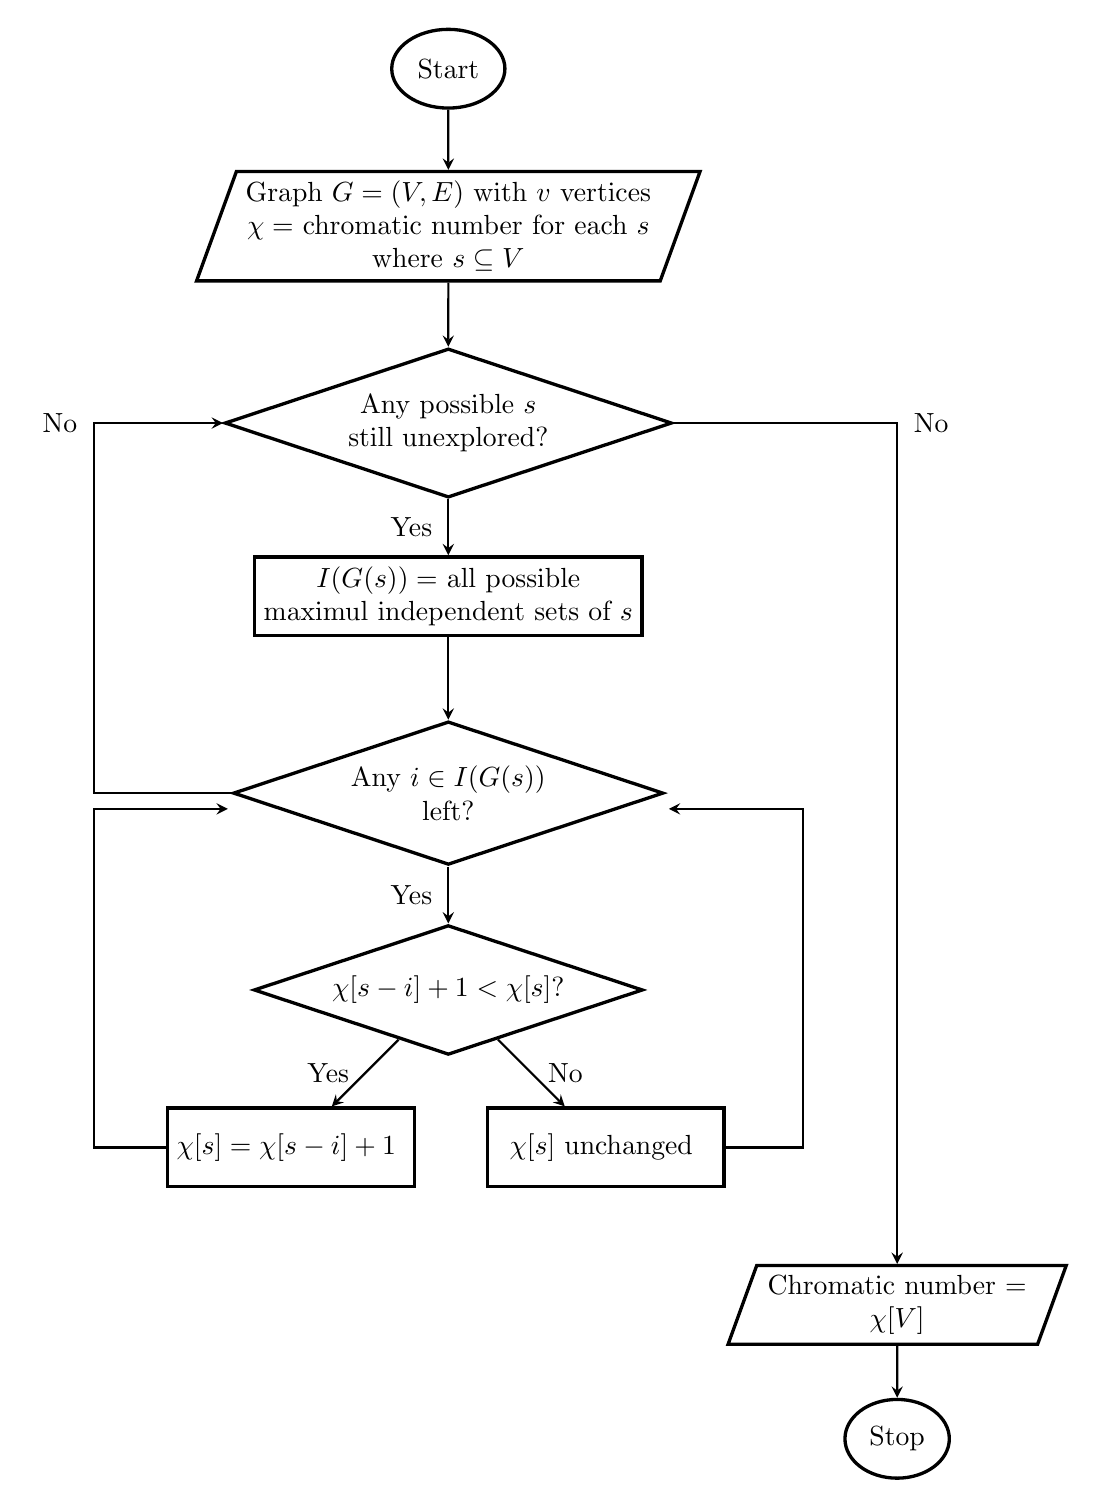
\begin{tikzpicture}
					
					\node[startstop, flow-highlight-on=<1>,
					] (start) {Start};
					
					\node[io, flow-highlight-on=<1>,
					below of = start, align=center, yshift=-1.0cm] (in) {
						Graph $G = (V,E)$ with $v$ vertices \\
						$\chi = $ chromatic number for each $s$ \\ where $s \subseteq V$ 
					};
					
					\node[decision, flow-highlight-on=<2>, flow-highlight-on=<9>, below of = in, yshift=-1.5cm, align=center] (exit_con) {Any possible $s$\\still unexplored?};
					
					\node[process, flow-highlight-on=<2>, 
					below of = exit_con, yshift = -1.2cm, align=center] (def_i){
						$I(G(s)) = $ all possible \\maximul independent sets of $s$
					}; % YO YO YO 
					
					\node[decision, flow-highlight-on=<3-8>, 
					below of = def_i, yshift = -1.5cm, align=center] (pick_i) {
						Any $i \in I(G(s))$\\left?
					};
					
					\node[decision, flow-highlight-on=<3-8>, 
					below of = pick_i, yshift = -1.5cm] (color_check) {$
						\chi[s-i]+1 < \chi[s]?
						$};
					
					\node[process, flow-highlight-on=<4>, flow-highlight-on=<6>, below of = color_check, yshift = -1.0cm, xshift = -2cm, align=center] (new_color) {
						$ \chi[s] = \chi[s-i] + 1 $
					};
					
					\node[process, flow-highlight-on=<8>, below of = color_check, yshift = -1.0cm, xshift = 2cm, align=center] (old_color) {
						$ \chi[s] $ unchanged
					};
					
					\node[io, flow-highlight-on=<9>, below of = old_color, yshift = -1.0cm, xshift = 3.7cm,, align=center] (out) {
						Chromatic number = \\
						$\chi[V]$
					};
					
					\node[startstop, flow-highlight-on=<9>, below of = out, yshift=-0.7cm] (exit) {Stop};
					
					\draw[arrow] (start) -- (in);
					\draw[arrow] (in) -- (exit_con);
					\draw[arrow] (exit_con) -| node[label,right] {No} (out);
					\draw[arrow] (exit_con) -- node[label, left] {Yes} (def_i);
					\draw[arrow] (def_i) -- (pick_i);
					\draw[arrow] (pick_i) -- +(-4.5,0) |- node[label, left]{No} (exit_con) ;
					\draw[arrow] (pick_i) -- node[label, left]{Yes} (color_check);
					\draw[arrow] (color_check) -- node[label,left] {Yes} (new_color);
					\draw[arrow] (color_check) -- node[label, right] {No} (old_color);
					\draw[arrow] (new_color) -- +(-2.5,0) |-  +(-0.80, 4.3) ;
					\draw[arrow] (old_color) -- +(+2.5,0) |-  +(+0.80, 4.3) ;
					
					\draw[arrow] (out) -- (exit);
					\end{tikzpicture}
				}
			\end{column}
		\end{columns}
		
	\end{frame}
	
	\begin{frame}{Complexity \& Limitations}
		\begin{itemize}
			\item Time Complexity: $O(2.4423^n)$\pause \vspace{10pt}
			\item Modifications by \textbf{Epstein} and \textbf{Byskov} lowers complexity to $O(2.4023^n)$ \pause \vspace{10pt}
			\item All algorithms require exponential space
		\end{itemize}
	\end{frame}
	
	% 	\section{Second Section}
	% 	\begin{frame}{Second Section: Frame 1}
	% 		\begin{figure}[h]
	% 			\centering
	% 			\caption{This caption is at the top}
	% %			\includegraphics[scale=0.4]{graph.png}
	% 			\label{fig:1}
	% 			%\caption{This is figure 1.}
	% 		\end{figure}
	% 	\end{frame}
	
	
	\section{Applications}
	\begin{frame}{Map Coloring}
		\begin{columns}
			\column{0.5\textwidth}
			\centering
			\begin{figure}
				\centering
				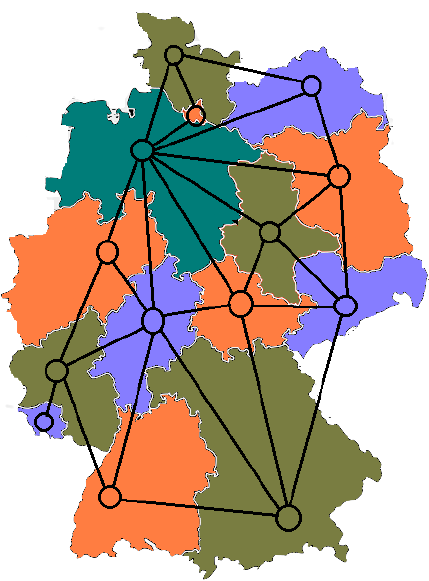
\includegraphics[scale=0.3]{diagrams/maps.png}
				%   \caption{Map Coloring}
				\label{fig:maps}
			\end{figure}
			\column{0.5\textwidth}
			\centering
			Coloring geographical maps of countries or states
		\end{columns}
	\end{frame}
	
	\begin{frame}{Register Allocation}
		\begin{figure}
			\centering
			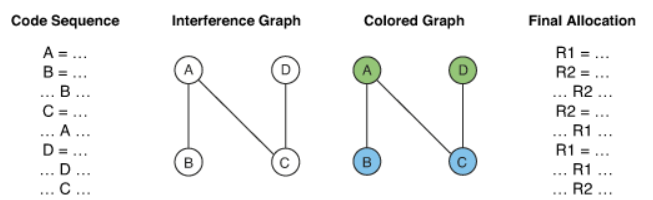
\includegraphics[scale=0.5]{diagrams/register_cropped.png}
			%   \caption{Map Coloring}
			\label{fig:regs}
		\end{figure}
		\vspace{1cm}
		\centering
		Assigning variables onto CPU registers
	\end{frame}
	
	\begin{frame}{Scheduling Tasks}
		\begin{figure}
			\centering
			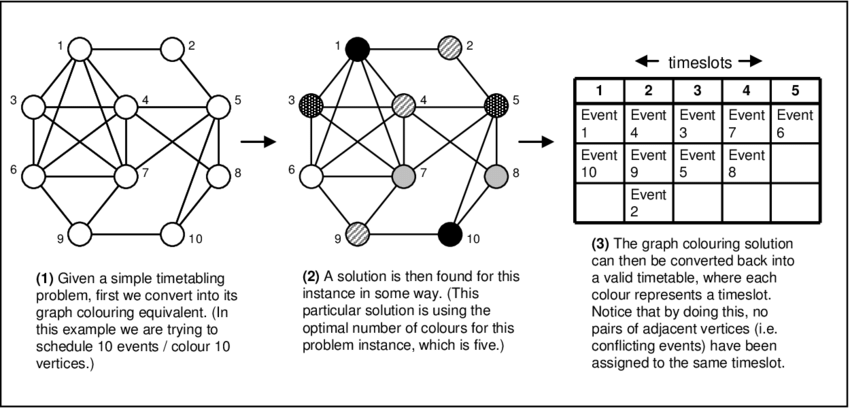
\includegraphics[scale=0.3]{diagrams/scheduling.png}
			%   \caption{Map Coloring}
			\label{fig:schedule}
		\end{figure}
		\centering
		Assigning timeslots with constraints \cite{article}
	\end{frame}
	
	{
		\setbeamertemplate{navigation symbols}{}
		\setbeamertemplate{footline}{} 
		\begin{frame}{Bibliography}
			\nocite{*}
			\printbibliography
		\end{frame}
	}
	
	{
		\setbeamertemplate{navigation symbols}{}
		\setbeamertemplate{footline}{} 
		\begin{frame}{The End}
			\centering
			\LARGE
			\textit{Thank you!}\\
			\vspace{10pt}
			\tiny
			Any Questions?
		\end{frame}
	}
	
	% %EFFECTS DEMO
	% \begin{frame}{Second Section: Frame 2}
	% This is a sample line of text.
	
	% \begin{itemize}
	%  \item<1-> Text visible from slide 1 
	%  \item<2-> Text visible from slide 2
	%  \item<3> Text visible on slide 3
	%  \item<4-5> Text visible on slides 4 and 5
	%  \item<5-> Text visible from slide 5
	%  \item<6-> Text visible from slide 6
	% \end{itemize}
	% \end{frame}
	
	% %EFFECTS DEMO USING PAUSE
	% \begin{frame}{Second Section: Frame 3}
	%  In this slide \pause
	
	%  the text will be partially visible \pause
	
	%  And finally everything will be there
	% \end{frame}
	
	% %TWO COLUMN SLIDE
	% \begin{frame}{Second Section: Frame 4}
	
	% \begin{columns}
	% \column{0.5\textwidth}
	% This is a text in the first column.
	% $$E=mc^2$$
	% This is a list.
	% \begin{itemize}
	% \item First item
	% \item Second item
	% \end{itemize}
	
	% \column{0.5\textwidth}
	% This text will be in the second column.
	% This is a nice looking
	% layout in some cases.
	% \end{columns}
	% \end{frame}
	
	% %BLOCK AND ALERT COMMANDS
	% \begin{frame}{Second Section: Frame 5}
	
	% In this slide, some important text will be
	% \alert{highlighted} because it's important.
	
	% \begin{block}{Remark}
	% Sample text
	% \end{block}
	
	% \begin{alertblock}{Important theorem}
	% Sample text in red box
	% \end{alertblock}
	
	% \begin{examples}
	% Sample text in green box. 
	% \end{examples}
	% \end{frame}
	
\end{document}